\documentclass{article}

% Set the margins to not be ridiculous
\usepackage[margin=0.75in]{geometry}
% Put space between paragraphs
\usepackage{parskip}
% For using images
\usepackage{graphicx}
\graphicspath{{gfx/}}

\newcommand{\photo}[3]{
      \begin{center}
            \includegraphics[width=#3in]{photos/#1/#2}
      \end{center}
}

\begin{document}

\def\han{Hanayama}
\def\cc{counter-clockwise}

\title{\han{} Puzzle Solutions Guide}
\author{Dan Whitman}
\date{}

\maketitle

\section{Valve (Level 4)}

\newcommand{\valvediagram}[1]{
      \begin{center}
            \includegraphics[width=1.3in]{#1}
      \end{center}
}
\def\vhalf{Valve half}
\def\hhalf{\han{} half}

\photo{valve}{puzzle}{1.5}

\subsection{Overview}

The Valve device consists of the following components:
\begin{enumerate}
      \item The gold colored inner ring with a hexagonal interior.
      \item The gold colored outer ring with a hexagonal exterior.
      \item The silver colored \vhalf{} ring with ``VALVE'' printed on one side.
      \item The silver colored \han{} ring with ``HANAYAMA'' printed on one side.
\end{enumerate}
These components are shown below, disassembled, in the above order from left to right.
\photo{valve}{components-top}{2.5}
\photo{valve}{components-angle}{2.5}
Note that, in the fully assembled state, the ``VALVE'' and ``HANAYAMA'' labels on the half rings are on opposite sides of the puzzle, like the two sides of a coin.

\subsection{Internal Structure} \label{sec:valve:struct}

The entire puzzle is can be divided up into a circle consisting of six segments that correspond to the six sides of the hexagons on the inner and outer rings, and three layers.
This is most clearly observed at the sides of the half rings, the insides and outsides of which are shown, respectively, below spread out with orientations as it normally assembled in the puzzle.
\begin{center}
      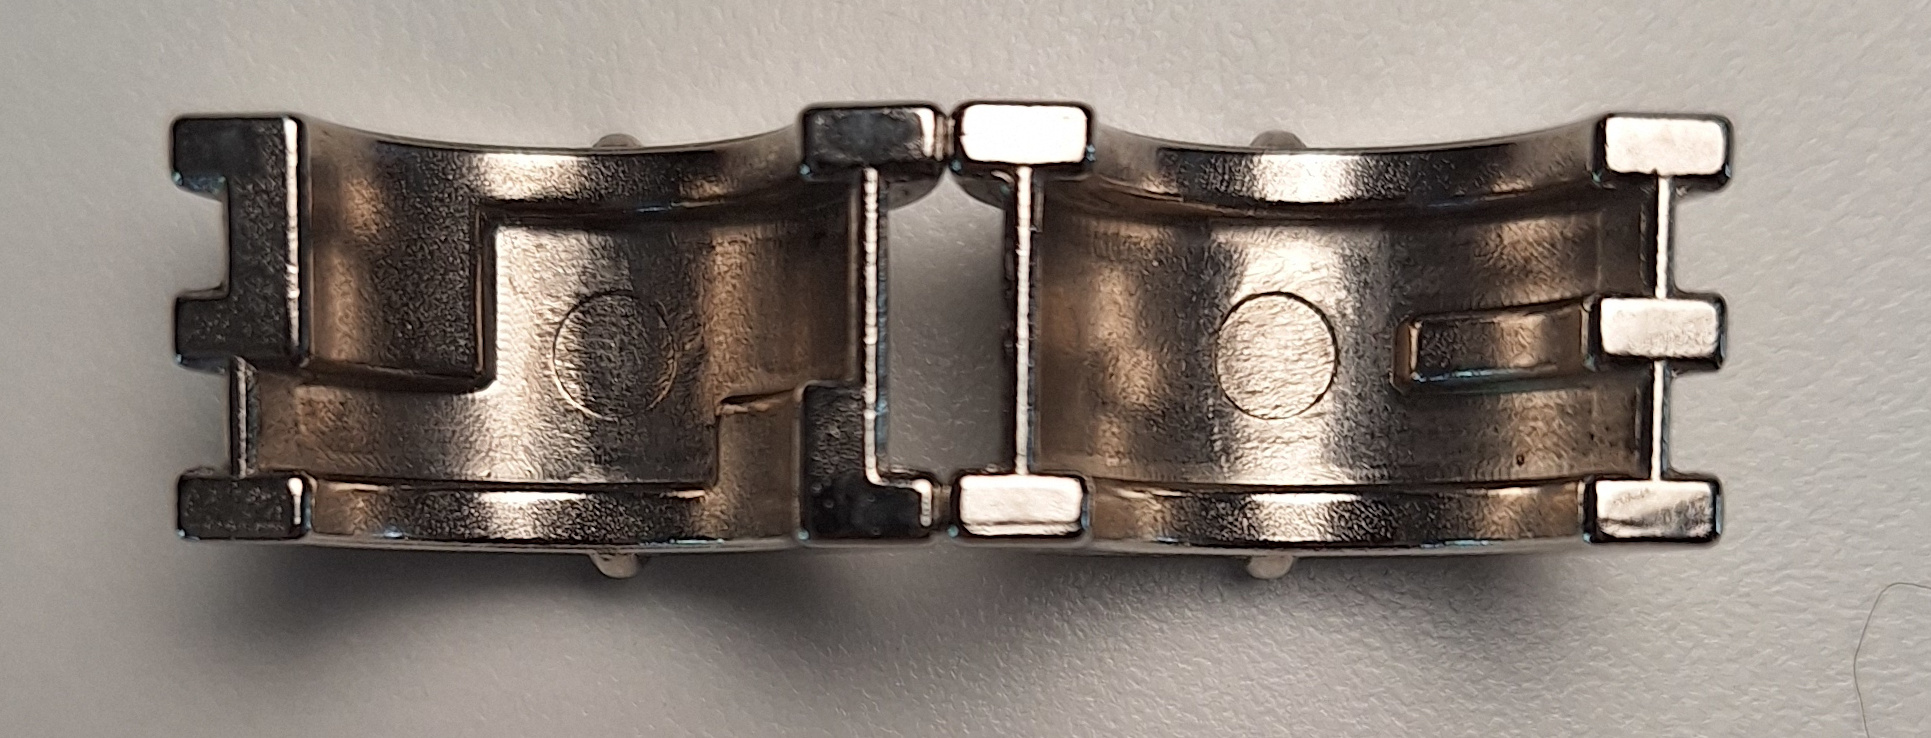
\includegraphics[height=0.955in]{photos/valve/halves-inside}
      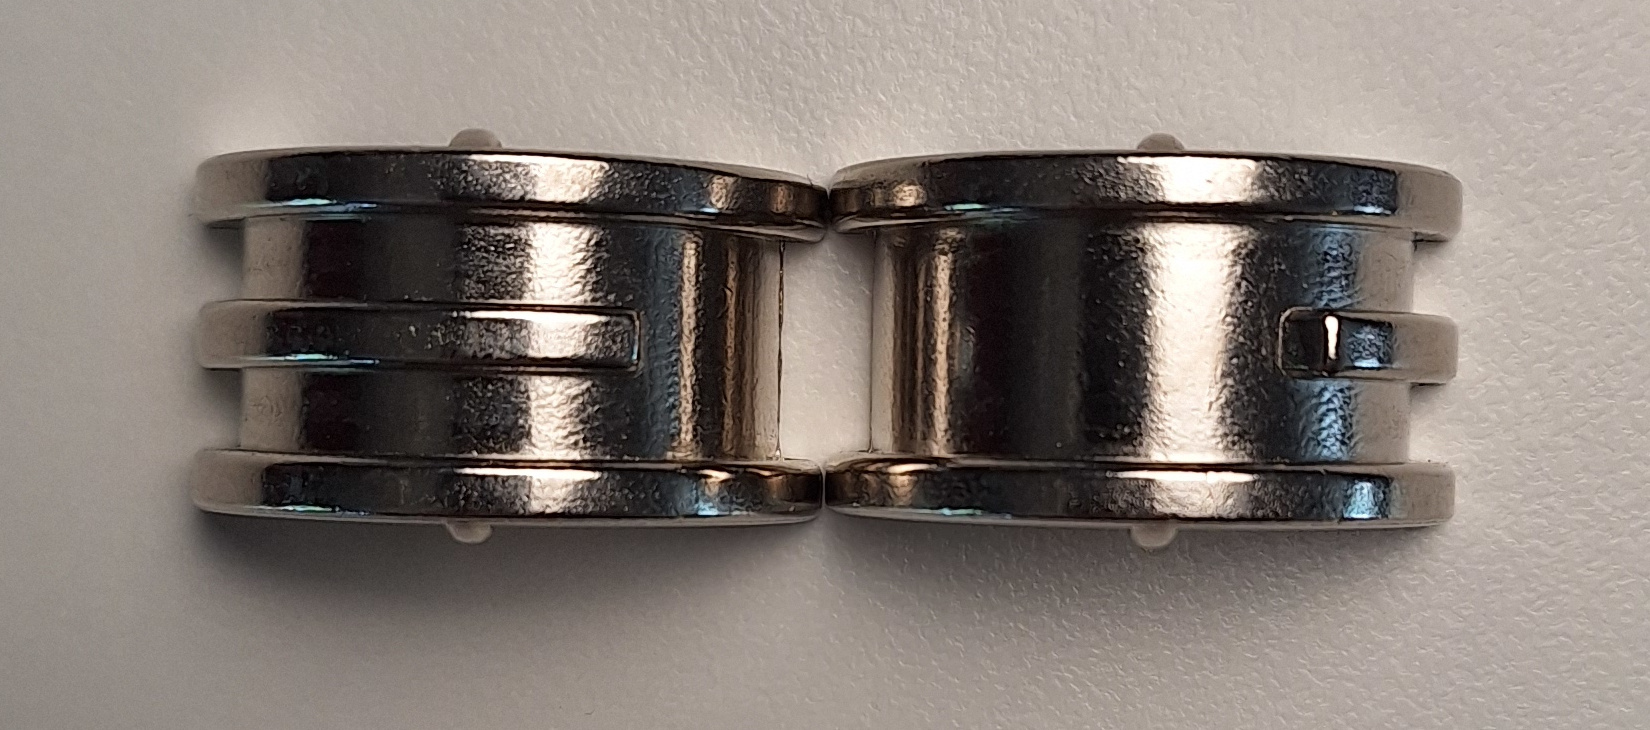
\includegraphics[height=0.955in]{photos/valve/halves-outside}
\end{center}
A software model of the Valve puzzle was created to aid in devising a solution, and the models for the insides and outsides are shown below, respectively.
\valvediagram{halves-00}
In the model, the black section with H's is the \hhalf{} ring and the white section with the V's is the \vhalf{} ring.
Note how the model corresponds with the above photos.

Both the inner and outer rings feature horizontal extrusions at various segments and layers that slide around in the grooves on the insides (for the inner ring) and outsides (for the outer ring) of the half rings.
This forms a kind of maze that has to be blindly navigated in order to disassemble and reassemble the puzzle.
It is not possible to fully view all the extrusions in a photo of the inner and outer rings, but they are shown below at an angle the renders some of them visible.
\photo{valve}{rings}{2.5}
These extrusions are also modeled in software, shown below, corresponding to the photo above.
\valvediagram{rings-00}
Here the inner ring is peach-colored and labeled with I's while the outer ring is pink and labeled with O's.

\subsection{Starting Position}

Though arbitrary, for the purposes of this analysis, we consider the silver colored half rings to be fixed, with the inner and outer rings rotating around them, independently of each other.
For the starting position, hold the puzzle with the ``HANAYAMA'' label facing up and in the lower right corner, as this is the orientation such that gravity will best assist us.
Now, in this orientation, the outer ring has a single extrusion very close to the top of the device, which can be seen through the gaps between the half rings and between the half rings and the outer ring if they are shifted slightly to leave a gap.
Find this extrusion by rotating the outer ring around and note that it is aligned to one of the sides of the outer hexagon on the outer ring.

Rotate outer ring until the extrusion is in the upper left corner of the puzzle with the end aligned to the upper gap between the half rings.
In this position the one of the vertices of the outer ring hexagon will be at the very top, aligned with the upper gap between the half rings.
Rotate the inner ring clockwise (looking at the top from above) all the way until it stops.
The hexagon inside in the inner ring will be aligned with the hexagon outside the outer ring such that the corresponding sides are parallel.

This is the starting position we shall use.
A picture of this starting position is shown below with the corresponding model:
\photo{valve}{starting-position}{1.5}
\valvediagram{starting-00}
After every step the hexagons will be aligned in the same way and, in what follows, we refer to rotations by a certain number of \emph{segments}.
A segment refers to a single side of the hexagon so that, for example, a rotation clockwise one segment will rotate in that direction $360^\circ / 6 = 60^\circ$, or one sixth of a full rotation, such that the hexagon of the rotated ring looks the same as before.

\subsection{Disassembly}

From the starting position, the solution to disassemble the device is as follows:
\begin{enumerate}
      \item Rotate the inner ring all the way \cc{} two segments until it stops.
            \valvediagram{apart-01}
      \item Rotate the outer ring \cc{} one segment.The \hhalf{} should drop down one layer.
            \valvediagram{apart-02}
      \item Rotate the inner ring \cc{} one segment, until it stops.
            \valvediagram{apart-03}
      \item Push the \hhalf{} back up and the inner ring will move with it.
            Holding the \hhalf{} up, rotate the outer ring clockwise two segments.
            The \vhalf{} should drop down one layer.
            \valvediagram{apart-04}
      \item Rotate the inner ring clockwise by one segment until it stops.
            The \vhalf{} should drop down another layer, taking the inner ring along with it.
            \valvediagram{apart-05}
      \item Rotate the outer ring \cc{} by two segments, exposing the top extrusion of the outer ring.
            The \hhalf{} should drop down one layer.
            \valvediagram{apart-06}
      \item Rotate the inner ring \cc{} by one segment until it stops.
            The \hhalf{} should drop down another layer, joining the \vhalf{} and taking the inner ring with it.
            \valvediagram{apart-07}
      \item Rotate the outer ring clockwise by one segment.
            The \vhalf{} should drop down by another layer.
            \valvediagram{apart-08}
      \item Rotate the inner ring clockwise by one segment until it stops.
            The \vhalf{} and inner ring should then fall completely out from the outer ring and \hhalf{}, making the other half easy to remove as well.
            \valvediagram{apart-09}
\end{enumerate}

\subsection{Reassembly}

Reassembling the puzzle can be a bit tricky at first.
It may be helpful to review section~\ref{sec:valve:struct} now that the puzzle is apart, and the components can be inspected.
Of particular importance for the initial step of reassembly is how the model relates to the physical components.
\begin{enumerate}
      \item Fit and hold the inner ring along with the half rings according to the model below.
            The \hhalf{} should be on the right with its label facing up on the bottom, and the Valve left on the right with its label facing down, in the same general orientation as for the disassembly.
            \valvediagram{together-01}
            In the real world this looks like this:
            \photo{valve}{together-1}{1.5}
      \item Still holding the inner and half rings with one hand so that they do not fall apart, place the outer ring on top with the other hand with the two lower extrusions resting on the top of the \vhalf{}, shown below.
            \photo{valve}{together-2}{1.5}
      \item Still holding the inner and half rings together, turn the outer ring by three segments in either direction, that is $180^\circ$, so that the lower extrusions both rotate inside the \hhalf{}.
            The puzzle should now look as below:
            \photo{valve}{together-3}{1.5}
            The corresponding model state is:
            \valvediagram{together-03}
      \item Push the \vhalf{} up a layer (as far as it will go) and hold it there.
            Then rotate the inner ring \cc{} until it stops.
            This will lock things in place so that they will no longer fall apart if not held together.
            \valvediagram{together-04}
      \item Still pushing the \vhalf{} up as far as it will go, rotate the outer ring \cc{} one segment, which will lock the \vhalf{} up to the same layer as the \hhalf{}.
            \valvediagram{together-05}
      \item Pushing the \hhalf{} up all the way will move the inner ring along with it.
            Holding the \hhalf{} up, rotate the inner ring clockwise one segment until it stops, which raises the \hhalf{} up another layer.
            \valvediagram{together-06}
      \item Again, holding the \hhalf{} all the way up, rotate the outer ring clockwise two segments so that its exposed extrusion slides into the \hhalf{}, locking it all the way up.
            \valvediagram{together-07}
      \item Push the \vhalf{} up all the way, moving the inner ring along with it.
            Holding it up, rotate the inner ring \cc{} by one segment until it stops.
            This raises the \vhalf{} up a layer.
            \valvediagram{together-08}
      \item Holding the \vhalf{} up to be level with the \hhalf{}, rotate the outer ring \cc{} by two segments.
            This will drop the \hhalf{} along with the inner ring down by a layer.
            \valvediagram{together-09}
      \item Allowing the \hhalf{} to be dropped down, rotate the inner ring clockwise by one segment until it stops.
            \valvediagram{together-10}
      \item Holding the \hhalf{} up, rotate the outer ring clockwise by one segment, locking the \hhalf{} up into place, level with the \vhalf{}.
            \valvediagram{together-11}
      \item Rotate the inner ring clockwise two segments until it stops.
            The puzzle is now back in its starting position.
            \valvediagram{starting-00}
\end{enumerate}
\end{document}
